\section{Consegna, inoltro e instradamento}

    In questo capitolo scopriremo come funziona effettivamente un router. Siamo ancora nello strato di rete, ovviamente.
    
    \vspace{3mm}
    
    Una \textbf{consegna} è definita come la gestione del pacchetto da parte dello strato di rete. 
    
    E' detta \textit{diretta} se chi riceve il pacchetto è sulla stessa rete di chi lo spedisce ed è realizzata dallo strato di collegamento. 
    
    E' detta \textit{indiretta} se chi riceve il pacchetto è su una rete diversa dalla rete di partenza del pacchetto, rendendo necessario attraversare un router.
    
    \vspace{3mm}
    
    Un \textbf{inoltro} è definito come la consegna del pacchetto al prossimo nodo del percorso verso la destinazione. 
    
    E' un'operazione necessaria alla consegna indiretta. Un router consulta la propria tavola di routing e trova l'indirizzo del prossimo router verso la destinazione finale, e cioè su quale interfaccia in uscita il paccheto debba essere inoltrato.
    
    \vspace{3mm}
    
    L'\textbf{instradamento} è definito come la costruzione o aggiornamento delle tavole di routing.
    
    \subsection{Tavole di routing}
    
        Le tavole di routing possono essere statiche o dinamiche.
        
        \vspace{3mm}
        
        Le \textbf{tavole di routing statiche} contengono informazioni inserite manualmente e sono difficili da gestire se non su reti molto piccole.
        
        Le \textbf{tavole di routing dinamiche} sono aggiornate periodicamente ogni qualvolta si verifica un cambiamento nella topologia della rete, come ad esempio la rimozione di un router o il malfunzionamento di un canale di comunicazione. L'aggiornamento utilizza i protocolli \textit{RIP}, \textit{OSPF} o \textit{BGP}.
        
        \vspace{3mm}
        
        Nella tavola di routing viene mantenuto un numero variabile di informazioni. Ad esempio, si potrebbe inserire nella tavola di routing l'intero percorso verso la destinazione finale; in alternativa, si potrebbe inserire una porzione di percorso (ad esempio fino al prossimo hop, cioè al prossimo router).
        
        \vspace{3mm}
        
        Mantenere il percorso completo è una scelta poco efficiente.
        
        Mantenere, invece, solo l'indirizzo del \textit{next-hop} permette di costruire tabelle più snelle. Tuttavia, anche questa soluzione è poco efficiente.
        
        \vspace{3mm}
        
        Allora si elabora una terza soluzione - detta di \textit{aggregazione} - che non prevede l'inserimento di tutte le possibili destinazioni finali (cioè gli host), bensì solo di tutte tutte le possibili reti. In termini pratici, se una rete ha 1000 host, la corrispondente tavola di routing conterrà una sola riga e non 1000.
        
        \vspace{3mm}
        
        Anche usando una riga per ogni possibile rete di destinazione finale, e un solo indirizzo di next-hop, le tavole di routing di Internet risulterebbero ancora inefficienti. Pertanto, le tavole di routing conterranno solo una lista parziale delle possibili reti di destinazione. Per tutte le reti non presenti nella tavola di routing ("\textit{il resto di Internet}") deve essere definita una \textbf{rotta di default} sulla quale inoltrare i pacchetti.
        
        \vspace{3mm}
        
        Quando un router riceve un pacchetto, deve consultare la sua tavola di routing per capire dove spedire tale pacchetto. Il primo step è estrarre l'indirizzo di destinazione del pacchetto; il secondo step è accedere, appunto, alla tavola di routing per cercare la riga che fornisce informazioni sulla rotta per quell'indirizzo.
        
        Osserviamo che la tavola di routing contiene almeno 4 informazioni: la maschera $/n$; la rete di destinazione; l'indirizzo per il prossimo router (hop), e l'interfaccia di rete sulla quale intradare i dati.
        
        In aggiunta, una tavola può anche contenere dati opzionali: la flag (indica se il next-hop è funzionante, su un'altra rete, è l'host di destinazione, etc); un contatore (indica il numero di connessioni che usano questo percorso), e un valore di pacchetti spediti (indica il numero di pacchetti spediti verso questo next-hop).
        
        \begin{center}
            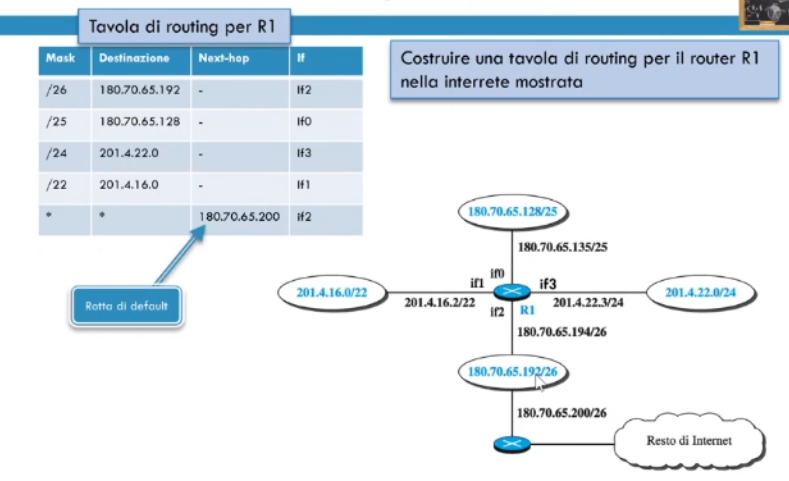
\includegraphics[scale=0.4]{images/TavolaRoutingEsempio.png}
        \end{center}
        
        Le entry sono ordinate in base alla maschera in modo decrescente.
        
        \vspace{3mm}
        
        Un'operazione di inoltro di un pacchetto che arriva al router R1 nella configurazione precedente e che è destinato all'indirizzo IP 201.4.22.35 è definita come segue.
        
        Il router controlla se la prima riga della tavola di routing è quella giusta, applicando la maschera $/26$ all'indirizzo di destinazione 201.4.22.35. Si otterrà l'indirizzo di rete $201.4.22.0$, che non corrisponde all'indirizzo di rete della prima riga. Pertanto questa riga non ci dà informazioni per inoltrare il pacchetto.
        
        L'operazione viene ripetuta per la seconda riga, e ancora una volta per la terza. La terza riga è quella giusta: il prossimo hop del pacchetto è proprio l'indirizzo di destinazione attraverso l'interfaccia IF3. L'indirizzo di destinazione e il numero dell'interfaccia vengono passati al protocollo ARP.
        
    \subsection{Aggregazione di indirizzi}
    
        Il concetto di \textbf{aggregazione}, che permette di riportare nella tavola di routing solo l'indirizzo della rete anziché dei singoli host, può essere usato per raggruppare - in maniera ancora più efficiente - più reti che condividono il next-hop, e quindi raccogliere più reti in una singola riga.
        
        \begin{center}
            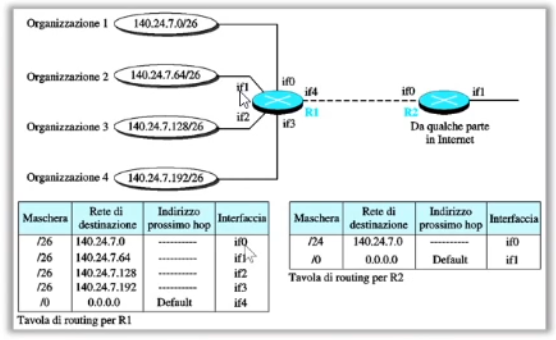
\includegraphics[scale=0.5]{images/Aggregazione.png}
        \end{center}
        
        L'aggregzione può essere gerarchica. Nei primi capitoli abbiamo parlato di ISP: osserviamo che ogni ISP utilizza il proprio livello di aggregazione. Per capire cosa significa, ricordiamo che ad un ISP locale viene assegnato un blocco di indirizzi - ora, è chiaro che non è necessarioche  tutti gli host e le reti raggiungibili da questo ISP all'interno di ogni singolo router dell'ISP stesso, ma aggiungo una sola riga che indica il next-hop relativo all'ISP.
        
        \vspace{3mm}
        
        Un modo per consultare le informazioni di routing sono i comandi \textit{netstat} e \textit{ifconfig}. Per più informazioni, cerca su Google.
        
    \subsection{Protocolli di routing}
    
        Un protocollo di routing è un insieme di regole che permettono ai router di una rete di scambiarsi informazioni riguardanti i cambiamenti circa la rete. Ricordiamo che un router è connesso almeno a 2 reti. Il compito principale di un router è quello di riceve un pacchetto e passarlo ad un'altra rete; la decisione fondamentale è quindi 'a quale rete' passare il pacchetto, per la quale esistono numerosi criteri di ottimizzazione.
        
        Definire un percorso "ottimo" significa, nella maggior parte dei casi, assegnare un costo per il passaggio di un pacchetto attraverso una rete. Il costo di un percorso diventa così la somma dei costi dei passaggi attraverso le singole reti; un percorso ottimo, quindi, è un percorso che minimizza tale costo. Adesso provami l'ottimalità di Dijkstra e Kruskal.
        
        \vspace{3mm}
        
        Internet è suddivisa in sistemi autonomi (gruppi di reti). Il routing all'interno del sistema autonomo viene detto \textbf{routing intradominio}; il routing fra più sistemi autonomi viene detto \textbf{routing interdominio}. In genere, il routing intradominio utilizza il protocollo RIP (basato sul vettore delle distanze) e l'OSPF (basato sullo strato dei collegamenti). Il routing interdominio utilizza il protocollo BGP (basato sul vettore dei cammini).
        
        \begin{itemize}
            \item 
                \textbf{RIP (Routing Information Protocol).} Assegna un costo unitario al passaggio in ogni rete. Il costo è il numero di hop ed è basato sul vettore delle distanze.
            
            \item
                \textbf{OSPF (Open Shortest Path First).} Permette all'amministratore di assegnare un costo in funzione del servizio richiesto. Tramite l'OSPF si ottiene il massimo throughput e il minimo ritardo. Basato sullo strato dei collegamenti.
                
            \item
                \textbf{BGP (Border Gateway Protocol).} Non utilizza costi, ma si preoccupa solo di trovare una qualsiasi rotta. Può usare criteri di natura amministrativa. Ad esempio, un ISP può decidere di non instradare i propri pacchetti attraverso un ISP concorrente. Basato sul vettore dei cammini.
        \end{itemize}
        
        \subsubsection{RIP}
            
            Analizziamo l'algoritmo del vettore delle distanze, che il RIP usa ampiamente. E' importante per l'esame.
            
            \vspace{3mm}
            
            I nodi della rete possono essere pensati come a delle città in una certa area geografica e i collegamenti come a delle strade che connettono questa città.
            
            E' possibile raggiungere una qualsiasi città partendo da una qualsiasi altra città, a patto che vi sia una strada che le connetta. Il costo per andare da una città all'altra è la lunghezza della strada (dunque la distanza) che collega le due città. Ogni nodo gestisce un vettore (tavola) delle distanze minime verso ogni altro nodo. La tavola contiene anche informazioni per instradare il pacchetto.
            
            \begin{center}
                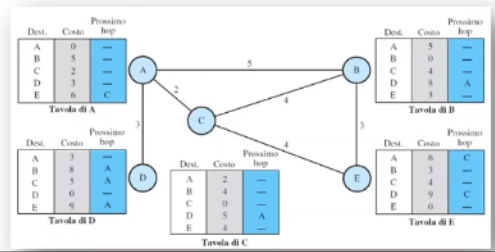
\includegraphics[scale=0.5]{images/Vector.png}
            \end{center}
            
            Inizialmente, la tabella contiene poche informazioni, cioè solo i nodi direttamente collegali. Le distanze verso i nodi che non sono direttamente collegati vengono considerate infinite.
            
            L'idea alla base del protocollo è lo scambio di informazioni fra nodi direttamente collegati. Nell'esempio, sebbene il nodo A non conosca la strada verso E, osserviamo il nodo C è direttamente collegato ad E, quindi C può condividere le informazioni nella propria tavola di routing col nodo A, in modo tale che A saprebbe raggiungere E.
            
            \begin{center}
                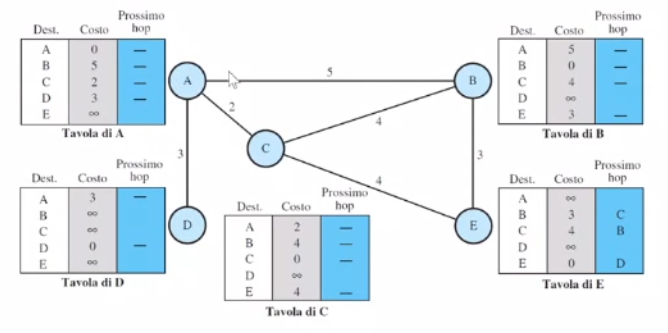
\includegraphics[scale=0.5]{images/Vector2.png}
            \end{center}
            
            Quindi ogni router invia la propria tavola periodicamente, e ogni router riceve una tavola, aggiornando la propria.
            
            Quando un nodo R riceve le inforamzioni della tavola di routing da un vicino V, deve aggiornare la propria tavola di routing. In particolare, se il nodo V dichiara di poter ragiungere una certa destinazione Z ad una distanza totale $x$ da V, il nodo R potrà raggiungere la stessa destinazione passando per V ad una distanza totale $x+d$, dove $d$ è la distanza fra R e V.
            
            \begin{center}
                $dist(R, V) = d$
                
                \vspace{2mm}
                
                $dist(V, Z) = x$
                
                \vspace{2mm}
                
                $dist(R, Z) = d+x$
                
                \vspace{2mm}
                
                $dist(S, Z) = d' + x$
            \end{center}
            
            Il prossimo hop per tutte le destinazioni e le distanze calcolate nel passo precedente dev'esser V. In altre parole, il nodo R costruisce una nuova tavola di routing in cui i costi sono calcolati come descritto nel passo precedente, e il prossimo hop per S ed R è il nodo V.
            
            \vspace{3mm}
            
            A questo punto, il nodo deve confrontare la tavoal costruita nelel deu fasi precedenti con la propria tavola di routing. Per effettuare l'aggiornamento, per ogni riga della tavola prende la seguente decisione: se la colonna del prossimo hop contiene 2 nodi diversi, allora viene scelta la riga col costo più piccolo; in caso di costi uguali, viene mantenuta la riga della tavola precedente; in atlernativa, se la colonna del prossimo hop contiene lo stesso nodo, allora viene scelta la riga della nuova tavola, anche se il costo dovesse essere più alto.
            
            \begin{center}
                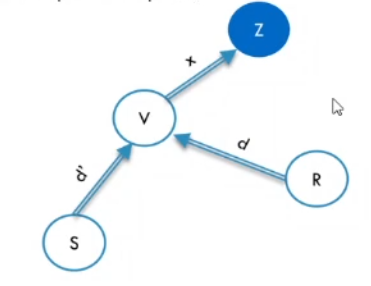
\includegraphics[scale=0.5]{images/Vector3.png}
            \end{center}
            
            Per motivare questa scelta, consideriamo il caso in cui un nodo C abbia in precedenza pubblicizzato la raggiungibilità del nodo X a una distanza di 3 e che il nodo A possa raggiungere il nodo X attraverso C.
            
            Se il nodo C invia una nuova tavola di routing in cui la distanza verso il nodo X è infinito, allora anche A dovrà aggiornare la distanza verso il nodo X, in quanto tale nodo dev'essere raggiungibile passando per C.
            
            \begin{center}
                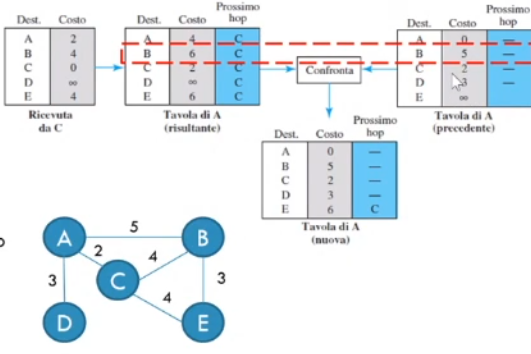
\includegraphics[scale=0.5]{images/Vector4.png}
            \end{center}
            
            \begin{center}
                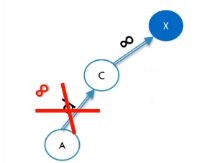
\includegraphics[scale=0.5]{images/Vector5.png}
            \end{center}
            
            In sintesi, ogni nodo spedisce la propria tavola di routing periodicamente o quando si verifica un cambiamento della tavola. La spedizione periodica della tavola avviene tipicamente ogni 30 secondi. Nel caso di guasto, la distanza verso i nodi che potevano essere raggiunti tramite il collegamento o il nodo adiacente diventa infinita. 
            
            Ogni qualvolta si verifica un aggiornamento della tavola di routing, la nuova tavola di routing viene inviata a tutti i vicini.
            
            \subsubsubsection{Instabilità}
            
                Un problema del routing basato sul vettore delle distanze è quello dell'\textbf{instabilità}.
                
                \vspace{3mm}
                
                Ad esempio, supponiamo che sia un nodo A che un nodo B sappiano raggiungere un nodo X.
                
                \vspace{3mm}
                
                Se il collegamento fra A ed X si rompe, il nodo A aggiornerà la propria tavola di routing nella quale viene scritto che X non è più raggiungibile (distanza infinita). A invia la tavola a B. Tuttavia, è possibile che B invii la propria tavola di routing PRIMA di riceve la nuova tavola di A. Questo significa che A riceve una tavola di routing in cui B dice di poter raggiungere X, pertanto A pensarà di poter raggiungere X non più direttamente come prima, ma attraverso B.
                
                \vspace{3mm}
                
                A questo punto, A spedisce il nuovo aggiornamento della propria tavola di routing a B. Il nodo B, ricevendo questa nuova tavola di routing in cui A dice di poter raggiungere X tramite B, aggiornerà la propria tavola di routing. Adesso B potrà raggiungere X tramite A ad una distanza maggiore della precedente, creando un ciclo.
                
                \vspace{3mm}
                
                Per uscire da questo loop, si potrebbe definire un "\textit{infinito finito}", cioè imporre un massimo alla distanza. 
                
                In alternativa, la soluzione degli \textbf{split horizon} prevede che l'intera tavola di routing non venga spedita ai vicini. Se, secondo la propria tavola di routing, B pensa che la strada ottima per X passi per A, allora B - quando spedirà la propria tavola ad A - non includerà la strada di X. 
                
                \vspace{3mm}
                
                Omettere questa informazione è ragionevole, ma crea un altro problema: normalmente, questi protocolli utilizzano delle scadenze per le informazioni nelle tavole di routing; quando un'informazione non viene aggiornata prima della scadenza, essa viene eliminata. Con la strategia dello split horizon, il nodo B volutamente non invia la distanza verso X ad A, e A non potrà quindi capire se B riceve i propri aggiornamenti.
                
                \vspace{3mm}
                
                Un'ulteriore strategia per ovviare a questo problema è il \textbf{poison reverse}, per la quale il nodo B continua a pubblicizzare ad A il percorso verso A, ma - anziché inserire la reale distanza verso X (che non interessa ad A) - inserisce un valore fittizio.
                
        \subsubsection{OSPF}
        
            Basato sullo strato dei collegamenti. E' importante per l'esame.
            
            \vspace{3mm}
            
            Nei protocolli di routing basati sullo strato dei collegamenti, ogni nodo costruisce una propria conoscenza dell'intera rete, cioè dei nodi, dei collegamenti e dei loro costi, e dell'usabilità dei collegamenti. Basandosi su questa conoscenza dell'intera topologia della rete, interpretando la rete come un grafo, ogni nodo può usare l'\textbf{algoritmo di Dijkstra} per costruire le tavole di routing.
            
            \vspace{3mm}
            
            Ogni nodo ha una conoscenza parziale della rete a cui è direttamente connessa. Mettendo insieme le conoscenze parziali, si ottiene una conoscenza globale della rete. Si vedino i collegamenti come archi pesati.
            
            \vspace{3mm}
            
            In particolare, i passi sono i seguenti.
            
            \begin{itemize}
                \item 
                    Creazione delle informazioni sullo strato di ogni collegamento da parte di ogni nodo; le informazioni vengono memorizzate in pacchetti denominati LSP (\textbf{Link State Packet}). 
                    
                    Ogni pacchetto LSP contiene l'identità del nodo che crea il pacchetto, l'elenco dei collegamenti di cui esso fa parte e il rispettivo costo, il numero di sequenza e l'istante di creazione. 
                    
                    I pacchetti LSP vengono generati in due occasioni: ogni volta che c'è un cambiamento della rete, e periodicamente (ogni 1-2 ore).
                
                \item
                    Disseminazione, fatta in modo efficiente ed affidabile, dei pacchetti LSP verso ogni altro nodo; tale disseminazione utilizza una tecnica detta di inondamento (\textbf{flooding}). 
                    
                    Il nodo che crea un LSP lo spedisce a tutti i suoi vicini. Quando un nodo X riceve un LSP da M, controlla se ha già altri LSP da M: se sì, ed il pacchetto è più recente del precedente, cancella il vecchio e spedisce una copia del pacchetto arrivato su ogni suoi collegamento, tranne quello da cui il pacchetto è arrivato; se no, lo ignora.
                    
                \item
                    Calcolo dell'albero dei cammini minimi da parte di ogni nodo (Dijkstra).
                    
                \item
                    Costruzione delle tavole di routing. La tavola di routing conterrà le colonne "nodo", "costo" e "next-hop".
            \end{itemize}
        
            In generale, l'OSPF divide il sistema autonomo in iù aree, ognuna delle quali riceve un identificativo e al quale viene applicato l'algoritmo degli strati dei collegamenti come sopra. Lungo i "bordi" di queste aree vi sono dei router, situati in aree dorsali, che si scambiano informazioni. Tali router sono detti router di dorsale.
            
            Il protocollo OSPF permette all'amministratore del sistema di assegnare un costo, chiamato metrica, a ogni percorso. La metrica è basata sul tipo di servizio (ritardo minimo, throughput massimo, etc). Un router potrà, dunque, avere più tavole di routing, ognuna per un certo servizio.
        
        \subsubsection{BGP}
            
            Basato sul vettore dei cammini. Non è richiesto nello specifico all'esame.
            
            \vspace{3mm}
            
            E' simile al vettore delle distanze, ma si spedisce l'intero cammino (senza usare metriche) e si evitano i cicli. Ogni sistema autonomo ha uno o più router portavoce che formano una rete logica e si scambiano informazioni di raggiungibilità. 
            
            Ognuno di questi router gestisce una propria tavola di routing e scambia le informazioni contenute nella tavola di routing con gli altri portavoce.
            
            \vspace{3mm}
            
            In ogni caso, ha due varianti: I-BGP (permette al portavoce di comunicare coi router interni) e E-BGP (per far comunicare portavoce di sistemi autonomi differenti).
            
            Inoltre, il BGP divide i sistemi autonomi (AS) in due categorie: AS terminali (con una sola connessione verso un altro AS) e AS di transito (con più connessioni verso altri AS).
            
            \vspace{3mm}
            
            Ogni router all'interno di un AS sa come raggiungere tutte le reti nel suo AS, ma non sa come raggiungere le reti in un altro AS. I router di confine eseguono i tre protocolli di instradamento: interdominio, E-BGP e I-BGP.